% Chapter Template

\chapter{Grundlagen} % Main chapter title

\label{Chapter4} % Change X to a consecutive number; for referencing this chapter elsewhere, use \ref{ChapterX}

\lhead{Chapter 4. \emph{Grundlagen}} % Change X to a consecutive number; this is for the header on each page - perhaps a shortened title

%-----------------------------------
%	THEORIE
%-----------------------------------

\section{Grundlagen und Definitionen}
In diesem Kapitel werden wichtige Begriffe vorgestellt, die im Verlauf der weiteren Arbeit von Bedeutung sind.

%-----------------------------------
%	WORKFLOW CASES
%-----------------------------------
\subsection{Prozess Schemata und Instanzen}

Ein Prozessschema \textbf{W = $\{T,D\}$} mit n $\in \mathbb{N}$ ist eine Menge von Aktivitäten \textbf{T = $\{t_1,t_2,...,t_n\}$} und einer Menge \textbf{D} von Abhängigkeiten, welche bestimmen, in welcher Reihenfolge die einzelnen Aktivitäten ausgeführt werden bzw von welchen Parametern abhängt, ob sie ausgeführt werden müssen, oder nicht. Die Menge der Aktivitäten muss mindestens eine Startaktivität haben, kann aber mehrere terminierende Aktivitäten beinhalten, die gleichberechtigt den Prozess abschließen.
$t_{ij}$ bezeichnet hierbei die Aktivität $t_j$ aus dem Prozessschema $W_i$. \\

\begin{figure}[ht]
	\centering
  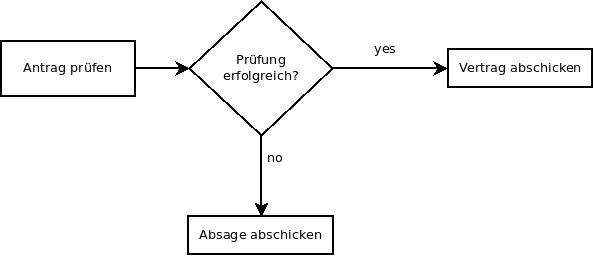
\includegraphics[width=0.7\textwidth]{Figures/sampleW}

\small Ein einfaches Beispiel für das Schema eines Prozesses mit einem Start und zwei möglichen finalen Aktivitäten. Abhängig von dem Ergebnis der Prüfung wird entweder ein Vertrag vorbereitet oder eine Absage verschickt.
	\caption{einfaches Beispiel eines Prozessschemas}
	\label{fig2}
\end{figure}

Ein Prozessschema kann mehrere Instanzen besitzen, die mit \textbf{W$_i^k$} gekennzeichnet werden.
Eine Prozessinstanz $W_i^k$ ist eine Menge von Instanzen $T_i^k$ der zugehörigen Aktivitäten. Dabei ist $|T_i| \subseteq |T|$ eine Teilmenge aller möglichen Aktivitäten des zugehörigen Schemas, da einzelne Aktivitäten unter Umständen aufgrund der Abhängigkeiten nicht ausgeführt werden müssen.


%-----------------------------------
%	ACTIVITIES TASKS
%-----------------------------------
\subsection{Aktivitäten}
\label{sec:activities}
Eine Aktivität ist ein atomares Event, dh. eine in sich abgeschlossene Aufgabe im Kontext eines Prozesses. Sie haben eine definierte Menge von potentiellen Rollen und Nutzern, die die Erlaubnis besitzen, diese Aufgabe auszuführen. Sobald sie einem Nutzer zugewiesen wurde, kann kein weiterer Nutzer mehr die Aufgabe annehmen. Das bedeutet, dass jede Aktivität einen eindeutigen Nutzer und eine eindeutige Rolle hat, welcher sie ausgeführt hat.

Des weiteren besitzen die Aktivitäten einen eindeutigen Zeitstempel $\tau$, zu dessen Zeitpunkt sie ausgeführt wurden. Diese Zeitstempel bestimmen eine Ordnung $<T, \leq>$. Es gilt nämlich $t_1 < t_2 $, wenn $t_1$ vor $t_2$ ausgeführt wurde, dh. timestamp($t_1$) $<$ timestamp($t_2$).

Aktivitäten besitzen 7 verschiedene Zustände: \textit{new, scheduled, assigned, active, suspended, completed, aborted}. Die Aktivitäten werden durch \textbf{Events} von einem Zustand in den nächsten geführt. Die Übergänge können sehr fein gegliedert sein oder sich nur auf elementare \textit{Events} beschränken. In dieser Arbeit wird von 12 \textit{Event}-Typen ausgegangen: \textit{schedule, assign, reassign, start, complete, resume, suspend, autoskip, manualskip, withdraw, ate\_abort, pi\_abort}.

\begin{figure}[ht]
	\centering
  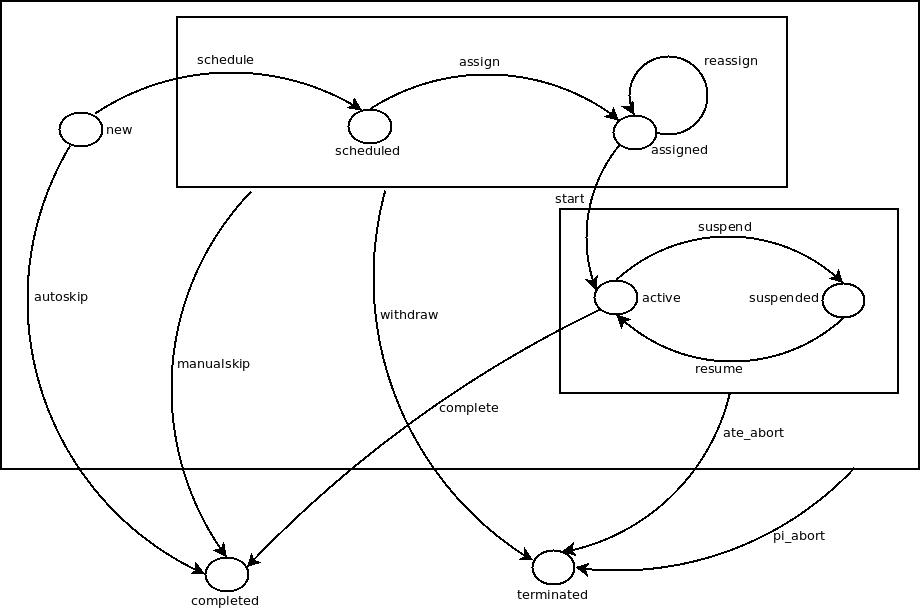
\includegraphics[width=0.9\textwidth]{Figures/Taskevents}

\small Eine Aktivität und ihre möglichen Zustände. Der Startzustand ist \textit{new}. Die neue Aktivität kann entweder sofort verworfen werden oder wird einem Nutzer zugewiesen und gestartet. Es gibt die Möglichkeit, die Aufgabe einem anderen Nutzer zuzuweisen oder zu pausieren und wieder zu starten. Aus jedem Zustand heraus kann die Aktivität abgebrochen werden.
	\caption{Aktivitäten und Events}
	\label{fig2}
\end{figure}
 

%-----------------------------------
%	ROLLENMODELL
%-----------------------------------
\subsection{Rollenmodell und Authorisierung}
Sei \textbf{T} = $\{t_1,t_2,...t_m\}$, $m\in\mathbb{N}$ eine Menge von Aktivitäten, \textbf{R} = $\{r_1,r_2,...t_n\}$, $n\in\mathbb{N}$ eine Menge von Rollen, und \textbf{U} = $\{u_1,u_2,...u_l\}$,$l\in\mathbb{N}$ eine Menge von Nutzern.

\begin{figure}[ht]
	\centering
  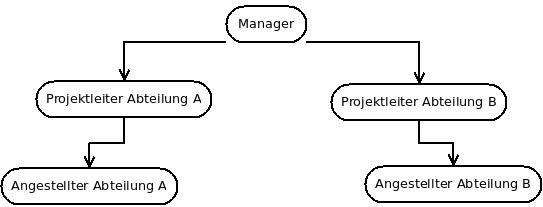
\includegraphics[width=0.7\textwidth]{Figures/Rollenmodell}
	\caption{Beispiel Rollenmodell}
	\label{fig:examplerolemodel}
\end{figure}

Eine \textbf{Authorisierung} ist eine Menge von potentiellen Nutzer und Rollen, denen es erlaubt ist, eine Aktivität auszuführen. Sie besteht aus den Tupeln $$\textbf{TR} = (T\times R)$$ und $$\textbf{UR} = (U\times R)$$
 welche eine n:m-Beziehung zwischen Aktivitätem und Rollen, bzw zwischen Nutzern und Rollen kennzeichnen. Das bedeutet, dass Nutzer mit Rollen in der Nutzer-Rollen Beziehung assoziiert werden und Aktivitätem mit Rollen in der Aktivitäten-Rollen Beziehung assoziiert werden.\\
Sei nun $$\textbf{R(t)} = \{r_m \in R: \exists(t_k, r_m) \in TR(t)\}$$
$$\textbf{U(t)} = \{u_n \in U: \exists(u_n, r_m) \in UR, r_m \in R(t)\}$$
Mit anderen Worten ist R(t) die Menge aller Rollen, die authorisiert sind, eine Aktivität t auszuführen und U(t) die Menge aller Nutzer, die authorisiert sind, einer Aktivität t zugeteilt zu werden.\\
Eine \textbf{Zuweisung} ist die konkrete Ausführung eines Tasks durch einen User.

Ein \textbf{hierarchisches Rollenmodell} ist eine geordnete Menge von Beziehungen zwischen Rollen $<R, \leq>$. Wenn $r_1, r_2 \in R$ und $r_1 < r_2$, dann dominiert die Rolle $r_2$ die Rolle $r_1$ in Bezug auf die organisatorische Rollenhierarchie. In Abb. \ref{fig:examplerolemodel} dominiert die Rolle 'Projektleiter' die Rolle 'Angestellter', das bedeutet, dass der 'Projektleiter' alle Tasks ausführen darf, die der Rolle 'Angestellter' zugeordnet wurde.
Die berechtigte Rolle und all ihre Elternrollen bis zur Wurzel können einem Task zugewiesen werden.

\cite{wolter_modeling_of_TBAC_in_BPMN}

%-----------------------------------
%	ZEITMODELL
%-----------------------------------
\subsection{Zeitmodell}
Das Zeitmodell ist ein Tupel \textbf{T} = ($\Tau;\leq$).\\
$\Tau$ ist eine Menge von \textit{Zeitpunkten} $\tau$ und $\leq$ eine total Ordnung auf $\Tau$.
Ein \textit{Zeitinterval} \\$\theta$ = $[\tau_a, \tau_b]$ (mit $\theta \in \Theta$ mit $\Theta$ = Menge aller Zeitintervalle) ist eine Menge von Zeitpunkten $\tau \in \Tau$ mit $\tau_a \leq \tau \leq \tau_b$.
Ein Zeitinterval $\tau' = [\tau_a, \tau_b]$ wird als leer bezeichnet, falss $\tau_b \leq \tau_a$. \cite{warner_inter_instance}

\textbf{TS} wird als die Menge aller Zeitpunkt-Variablen und Konstanten wie 30.07.1999, 14:55 definiert und \textbf{TP} bezeichnet die Menge aller Zeitspannen wie 3 Tage 5 Stunden, 5 Monate.\\
Es gilt: $$TP - TP = TS$$ und $$TP + TS = TP$$ Die Differenz zwischen zwei Zeitpunkten ist eine Zeitspanne ( 30.07.1999 - 25.7.1999 = 5D ) und die Summe von einem Zeitpunkt und einer Zeitspanne ist wieder ein Zeitpunkt ( 25.07.1999 + 5D = 25.07.1999 ).




%-----------------------------------
%	Event Logs
%-----------------------------------
\subsection{Event Logs}

EventLogs sind Abbildungen von Prozessen $W_i$ auf eine Teilmenge $E \subseteq W_i$. Ein EventLog kann durchaus unvollständig sein bzw Fehler beinhalten. Jedoch wird in dieser Arbeit von einer \textit{Closed World} ausgegangen, was bedeutet, dass eine Aktivität, die nicht geloggt wurde, auch nicht stattgefunden hat.

\begin{figure}[h!]
	\centering
  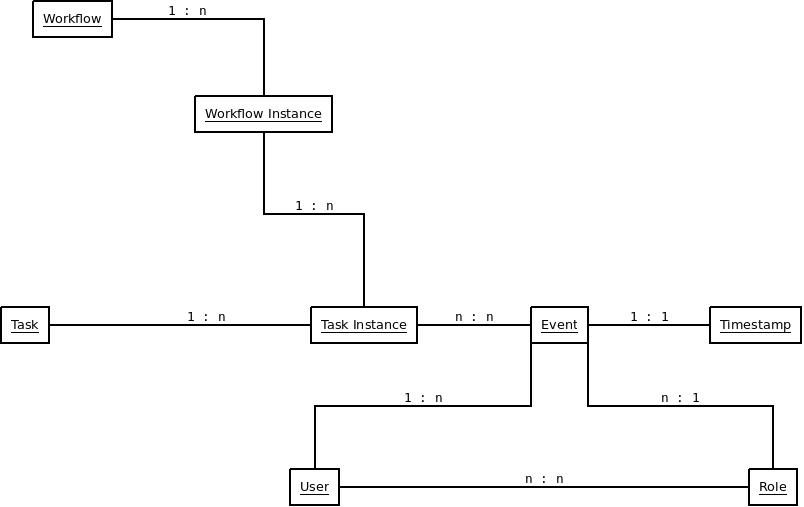
\includegraphics[width=0.9\textwidth]{Figures/WorkflowOntology}

\small Ein Prozessschema kann mehrere Instanzen haben, welche wiederrum aus Instanzen von mehreren Aktivitäten bestehen können. Die Instanz besitzt mehrere Events (\textit{start, complete,...}), die einen eindeutigen Zeitstempel, einen eindeutigen Nutzer und eine eindeutige ausführende Rolle besitzen. Der Nutzer hat im Moment der Ausführung ebenfalls eine eindeutige Rolle. Eine Aktivität kann zudem mehrere zusätzliche Attribute haben.
	\caption{Ontologie eines Prozesses}
	\label{fig:ontology}
\end{figure}

EventLogs repräsentieren die Instanzen eines Prozesses durch Auflistung der einzelnen Aktivitäten. In Tabelle \ref{tab:examplelog} wird ein exemplarischer Log dargestellt. Die \textit{caseID} kennzeichnet die Instanz des Prozesses, da ein Prozessschema mehrere Instanzen besitzen kann. Zu einer Prozessinstanz können mehrere Aktivitäten (hier \textbf{Task}) gehören, die jedoch einen eindeutigen Zeitstempel, Eventtypen, Nutzer und dessen Rolle haben. Zudem kann eine Aktivität beliebig viele zusätzliche Informationen besitzen, die in dieser Tabelle nur angedeutet werden.

\begin{table}[h!]
\footnotesize
  \centering
  \begin{tabular}{|c|c|c|c|c|c|c|}
  \hline
  caseID & Task & User & Role & Timestamp & EventType & DataAttributes\\
  \hline
  0 & Approach check &'Mark' &'Admin' &1999-12-13T12:22:15 & start&(amount, 3000)\\
  0 & Pay check & 'Theo' &'Azubi' &1999-12-13T12:22:16 & start&(amount, 3000Euro)\\
  1 & Approach check &'Lucy' & 'Azubi' &1999-12-13T12:22:17 &start&(customer, Max Muster)\\
  1 & Pay check &'Mark' & 'Admin' &1999-12-13T12:22:18 & abort&()\\
  0 & Revoke check & 'Theo' & 'Clerk' & 1999-12-13T12:22:19 & start&()\\
  \hline
  \end{tabular}
\\
Das ist nur ein Auszug und kein vollständiger Log. Es können auch weitere Daten vorhanden sein, die hier nicht dargestellt werden.
  \caption{Beispiel Log Einträge. }
  \label{tab:examplelog}
\end{table}

\section{Herleitung der Einschränkungen}


%-----------------------------------
%	Definition Constraints
%-----------------------------------

\subsection{Ein praktisches Beispiel}
\label{sec:exampleconstraints}

In diesem Kapitel werden verschiedene Arten von Einschränlungen und Regeln betrachtet.
Einschränkungen und Regeln sind Erwartungen, die aus dem Verlauf von vorhergehenden Aktivitäten resultieren. Einschränkungen und Regeln werden hier synonym verwendet.
Einschränkungen haben den Zweck Betrug, aber auch menschliches Versagen zu verhindern.
Um sich ein besseres Bild von Einschränkungen zu machen, betrachten wir vor der eigentlichen Analyse ein Beispiel, welches im Verlauf der Arbeit auf die Einhaltung der Regeln untersucht wird.

Der Prozess in Abbildung \ref{fig:Workflow} stellt die Bearbeitungsschritte eines Kreditantrages in einer Bank dar. In (T1 - Antrag empfangen) müssen zuerst alle erforderlichen Daten des Kunden aufgenommen werden. Daraufhin muss der Antrag geprüft werden, wie zum Beispiel die Kreditwürdigkeit des Kunden (T2 - Antrag prüfen). Sollte der gewünschte Betrag des Kredites 100000 Euro übersteigen, muss der Antrag zur Sicherheit von einer weiteren Person geprüft werden (T3 - Antrag prüfen). Nun muss entweder ein Vertrag vorbereitet werden (T4) oder, falls die Prüfung negativ verlaufen ist, ein Schreiben vorbereitet werden, welches den Antrag ablehnt (T5). Unabhängig von dem Ergebnis wird der Kunde zuletzt noch einmal kontaktiert (T6).
\begin{figure}[ht]
	\centering
  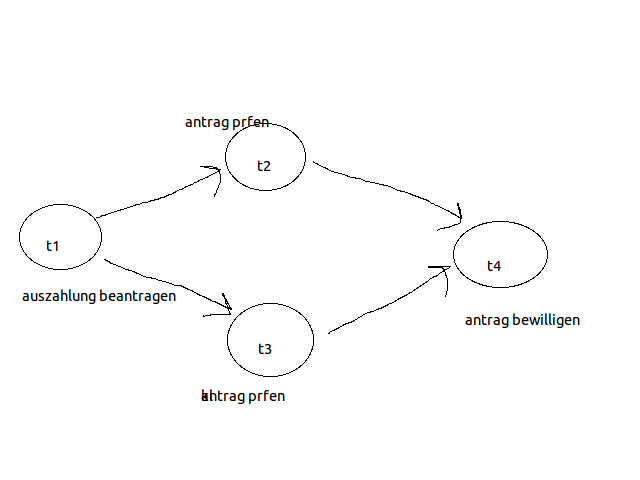
\includegraphics[width=0.9\textwidth]{Figures/Workflow}
	\caption{Bearbeitung eines Kreditantrags in der Bank}
	\label{fig:Workflow}
\end{figure}
\newpage
Um einen sicheren und reibungslosen Ablauf zu gewährleisten, werden folgende Anforderungen gestellt:

(C1) Der Kontakt mit Kunden (T1 und T6) muss durch den Kundenberater erfolgen.\\
(C2) Um den Kunden nicht zu lange warten zu lassen, sollte der Kunde spätestens 3 Tage nach erstem Kontakt über das Ergebnis informiert werden (timestamp(T6) $<$ timestamp(T1) + 3D).\\
(C3) Den Antrag annehmen (T1) und den Antrag prüfen(T2, T3) sollten von verschiedenen Personen erledigt werden (4 Augen Prinzip).\\
(C4) Ferner sollten auch die zwei Prüfungen von verschiedenen Mitarbeitern vollzogen werden. T3 muss durch den Bank Manager erfolgen.\\
(C5) Es dürfen keine Anträge von Verwandten geprüft werden.\\

(C6) Ein Mitarbeiter darf bei dem selben Kunden höchstens Kredite bis 100000 Euro prüfen.\\
(C7) Ein Mitarbeiterpaar darf höchstens 3mal gemeinsam an T1 und T2 arbeiten.\\

(C8) Wenn ein Mitarbeiter 5x einem Task zugewiesen wird und ihn dann abbricht, darf er nicht mehr an dem Task arbeiten.\\
(C9) Um zu verhindern, dass Fehler durch Überlastung passieren, darf jeder Mitarbeiter am Tag höchstens 100 Tasks bearbeiten.\\

%
% Arten von Constraints
%
\subsection{Arten von Einschränkungen}
\label{sec:ArtenConstraints}

Generell kann man Einschränkungen bezüglich des Verlaufs, zeitliche Einschränkungen, Abhängigkeiten von Parametern und Authorisierungsregeln unterscheiden. Jedoch sind sie nicht klar voneinander getrennt, sondern oft innerhalb einer Regel vermischt. Im folgenden werden die Arten von Regeln kurz erläutert.\\

\begin{figure}[ht]
	\centering
  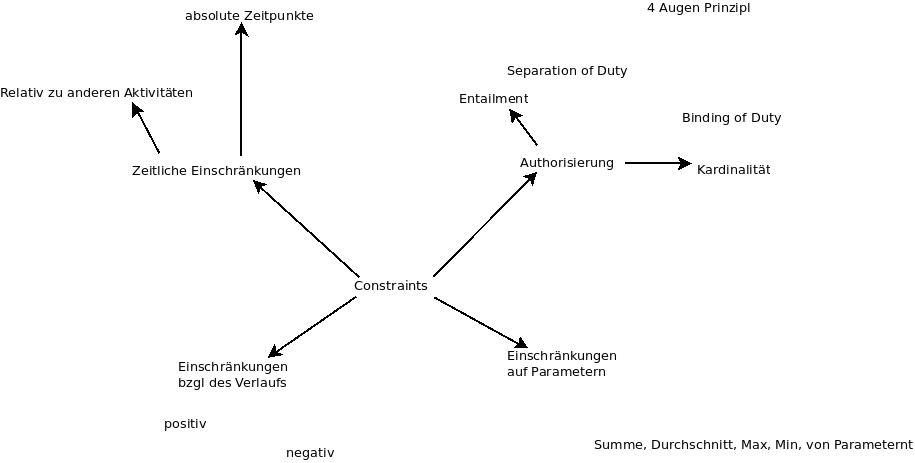
\includegraphics[width=0.9\textwidth]{Figures/Constraints}
	\caption{Typen von Einschränkungen und Regeln}
	\label{fig:constraints}
\end{figure}

\textbf{Zeitliche Beschränkungen}\\
\textbf{- absolute Einschränkungen}\\
Das sind Einschränkungen, die sich auf einen absoluten Zeitpunkt beziehen, wie zum Beispiel dass besondere Kredite nicht mehr vergeben werden dürfen, nachdem das Angebot erloschen ist. Sollte nach dem festgelegten Datum trotzdem dieser Kredit vergeben werden, stellt das einen Regelbruch dar.\\
\textbf{- relative Einschränkungen}\\
Relative Einschränkungen beziehen sich auf vorher erfüllte Aufgaben und schränken die weiteren für einen bestimmten Zeitraum ein.\\

\textbf{Einschränkungen auf Parametern}\\
Einschränkungen, die mit der Aggregation von Aktivitäten arbeiten, geben oft eine Grenze für einen Parameter in einem bestimmten Zeitraum vor. Diese Art der Einschränkungen ist häufig mit zeitlichen Einschränkungen verbunden.\\

\textbf{Entailment Constraint}\\
\textit{Entailment-Constraints} machen Aussagen darüber, in welcher Beziehung die Ausführenden zweier Aktivitäten zueinander stehen.
\textit{Rollenbasierte Entailment-Constraints} haben die Form $(R, \{t_1,t_2\}, pred)$ mit \textbf{R} als Teilmenge aller Rollen. Die Rollen aus R sind zugelassen, $t_1$ und $t_2$ auszuführen. \textit{pred} ist ein Prädikat aus der Menge $\{=, \neq,<, \leq,>, \geq \}$ und gibt an, in welchem Verhältnis gemäß der Rollenhierarchie die ausführenden Rollen zueinander stehen müssen.\\
\textit{Nutzerbasierte Constraints} $(U, \{t_1,t_2\}, pred)$ legen fest, welches Verhältnis die Nutzer in Bezug auf ihre Rollen bei der Ausführung von $t_1$ und $t_2$ haben müssen.
\cite{wolter_modeling_of_TBAC_in_BPMN} \cite{Entailment1} \cite{tan_consistency}

\textbf{Cardinality Constraints}\\
Kardinalitätseinschränkungen haben die generelle Form $(T, k, n_u, n_r)$ und besagen, dass eine Menge von Aktivitäten \textbf{T} von $n_u$ verschiedenen Personen und $n_r$ verschiedenen Rollen ausgeführt werden muss. Man unterscheidet zwischen \textit{lokalen} und \textit{globalen} Einschränkungen. \textit{Lokale} Einschränkungen beziehen sich auf verschiedene Instanzen der selben Aktivität in einer Prozessinstanz. Sie haben die Form $(t, k, n_u, n_r)$ und können zusätzlich eine Aussage darüber treffen, wieviele Instanzen einer Aktivität es geben muss (k). \textit{Globale} Kardinalitätseinschränkungen sind Einschränkungen auf die Instanzen von einer gegebenen Menge von Aktivitäten T in der selben Prozessinstanz.
\cite{wolter_modeling_of_TBAC_in_BPMN} \cite{Entailment1} \cite{tan_consistency}


\textbf{Separation of Duty}\\
Das Separation of Duty-Prinzip ist ein Speziallfall der Kardinalitätseinschränkungen und kann für zwei Aktivitäten $t_1$ und $t_2$ als $(\{t_1,t_2\},2)$ ausgedrückt werden. Das Separation of Duty Prinzip ist eine Form von Aufgabentrennung, in der kritische Aufgaben zerlegt werden und dann von verschiedenen Nutzern ausgeführt werden müssen.
\cite{SOD}\cite{SOD2}

\textbf{Binding of Duty}\\
\textit{Binding of Duty} - Aufgabenbindung ist das Gegenteil von \textit{Separation of Duty}, und ist ebenfalls ein Spezialfall von \textit{Cardinality Constraints}. Es hat die Form $(\{t_1,t_2\},1)$. Bei diesem Prinzip müssen zwei Aufgaben von der selben Person erledigt werden.


\textbf{Workflow Soundness}\\
Das sind Regeln, die allgemein den korrekten Ablauf eines Prozesses sicherstellen sollen. Diese Regeln beziehen sich im Allgemeinen nicht darauf, welcher Nutzer eine Aktivität ausgeführt hat (keine Authorisierungs-Einschränkungen) sondern betrachten die Tatsache, ob eine Aktivität zu einem korrekten Zeitpunkt oder in einem korrekten Zusammenhang ausgeführt wurde.

\subsection{Gültigkeitsbereich von Constraints}
\label{sec:rulecontext}
\textbf{Intra-Instanz}\\
Die meisten Ansätze beziehen sich auf Regeln, die in Bezug zu einer Prozessinstanz stehen. Hier gilt, dass die Prozessinstanz für alle Aktivitäten die selbe ist. Sollten zwei Aktivitäten zu verschiedenen Instanzen gehören, werden sie nicht gegeneinander betrachtet. Seien A und B zwei Aktivitäten, dann gilt A.caseID = B.caseID. 
\\
\textbf{Inter-Instanz}\\
Wie bereits erkannt wurde, reicht es nicht aus, nur Einschränkungen innerhalb eines Prozesses zu definieren, da sich eine kriminelle Handlung auch über mehrere Instanzen bemerkbar machen kann. Die Einschränkung von oben wird hier aufgehoben, es gilt jedoch noch, dass die betrachteten Tasks zum selben Prozessschema gehören müssen, dh A.case = B.case
\\
\textbf{Inter-Prozess}\\
Die Regeln beziehen sich auf alle Aktivitäten, unabhängig davon, zu welcher Prozessinstanz oder welchem Prozessschema sie gehören. Diese Einschränkungen betrachten häufig die Akkumulation von verschiedenen Aktivitäten, ihre Anzahl bzw Operationen auf die Aggregation ihrer Parameter.

